\documentclass[english,11pt]{article}

%PUT ALL THE PREAMBLES HERE
\usepackage[T1]{fontenc}
\usepackage[latin9]{inputenc}

% \makeatletter % to be able to overwrite package containing @
\usepackage{siunitx}
% \usepackage{subfig}
\usepackage{colonequals}
\usepackage[super]{nth}
\usepackage{algorithm}
\usepackage{amsmath}
\usepackage{amsthm}
\usepackage{amssymb}
\usepackage{tikz}
\usepackage{url}
\usepackage{float}
\usepackage{tabularx}
\usepackage{pbox}
\usepackage{tabulary}
\usepackage{breqn}
\usepackage{graphicx}
\usepackage{wrapfig}
\usepackage[font={small}]{caption}
\usepackage{enumitem}
\usepackage{physics}
\usepackage{lipsum}
\usepackage{mwe}
\usepackage{breqn}
\usepackage[noend]{algpseudocode}
\usepackage{subcaption}
\usepackage{graphicx}
\usepackage{enumitem}

\usepackage{hyperref}
\hypersetup{
    colorlinks,
    citecolor=black,
    filecolor=black,
    linkcolor=black,
    urlcolor=black
} % set up hyperlink for table of content
% \usepackage[]{algorithm2e}
% \SetKwInOut{Parameter}{Parameter}

\graphicspath{{./images/}{./}}

\newtheorem{claim}{Claim}
\newtheorem{theorem}{Theorem}
\newtheorem{lemma}{Lemma}
\newtheorem{remark}{Remark}
\newtheorem{corallary}{Corollary}
\newtheorem{conjecture}{Conjecture}
\newtheorem*{observation}{Observation}
\newtheorem*{myQuote}{Quote}
\newtheorem{fact}{Fact}
\newtheorem{definition}{Definition}
\newtheorem{assumption}{Assumption}
\newtheorem{example}{Example}
% \newtheorem{proof}{Proof}

\newcommand{\R}{\mathbb{R}}
\newcommand{\E}{\mathbb{E}}
\renewcommand{\P}{\mathbb{P}}
\newcommand{\I}{\mathbb{I}}

% \renewenvironment{proof}{{\bfseries Proof}}{\qed}

\makeatletter
\def\BState{\State\hskip-\ALG@thistlm}
\makeatother

\newtheorem*{theorem*}{Theorem}
\newcommand*{\vertbar}{\rule[-1ex]{0.5pt}{2.5ex}}
\newcommand*{\horzbar}{\rule[.5ex]{2.5ex}{0.5pt}}

\newcommand{\norms}[1]{\|#1\|_2^2}

\DeclareMathOperator*{\argmax}{arg\,max}
\DeclareMathOperator*{\argmin}{arg\,min}

\renewcommand{\norms}[1]{\|#1\|_2^2}
\newcommand{\la}{\langle}
\newcommand{\ra}{\rangle}

% Jari

\newtheorem{alg}{Algorithm}
% Maths
\newcommand{\N}{\mathbb{N}}
\renewcommand{\abs}[1]{\lvert #1 \rvert}
\renewcommand{\norm}[1]{\lVert #1 \rVert}
\newcommand{\snorm}[1]{\left\lVert #1 \right\rVert}
\newcommand{\deq}{\mathrel{\mathop:}=}
\newcommand{\eqd}{=\mathrel{\mathop:}}
\renewcommand{\grad}{\nabla}
\renewcommand{\d}{\partial}
%English
\newcommand{\cf}{\hbox{{cf.}}\xspace}
\newcommand{\deletia}{\ldots [deletia] \ldots}
\newcommand{\etal}{\hbox{{et al.}}\xspace}
\newcommand{\eg}{\hbox{{e.g.}}\xspace}
\newcommand{\ie}{\hbox{{i.e.}}\xspace}
\newcommand{\scil}{\hbox{{sc.}}\xspace} %scilicet: it is permitted to know
\newcommand{\st}{\hbox{{s.t.}}\xspace}
\newcommand{\wrt}{\hbox{{w.r.t.}}\xspace}
\newcommand{\etc}{\hbox{{etc.}}\xspace}
\newcommand{\viz}{\hbox{{viz.}}\xspace} %videlicet: it is permitted to see
\newcommand{\vs}{\hbox{{vs.}}\xspace}


\newenvironment{proof_sketch}{%
  \renewcommand{\proofname}{Proof Sketch}\proof}{\endproof}



\usepackage[margin=1in]{geometry}
 \usepackage{setspace}
% \setstretch{}
\usepackage{listings}

\lstset { %
    language=C++,
    backgroundcolor=\color{black!5}, % set backgroundcolor
    basicstyle=\footnotesize,% basic font setting
}

\begin{document}

\title{Computing Large Scale Linear Least Squares with SKiLLS}

\author{Zhen Shao}\maketitle

\section{Overview}

SKiLLS (SKetchIng-Linear-Least-Sqaures) is a C++ package for finding solutions to over-determined linear least square problems. SKiLLS uses a modern dimensionality reduction technique called sketching, and is particularly suited for large scale linear least squares where the number of measurements/observations is far greater than the number of variables. 

Mathematically, SkiLLS solves

\begin{align}
\min_{x \in \R^{d}} f(x): = \|Ax - b\|_2^2, \label{eq::problem}
\end{align}
where $A \in \R^{n\times d}$ and $b \in \R^{n}$ given. The matrix $A$ is allowed to be rank-deficient or nearly rank-deficient. 

\subsection{When to use SKiLLS}

Problem \eqref{eq::problem} frequently appears as a sub-problem in many computational and data science problems, for example, in many non-linear/general function minimisation routine linearises the problem and iteratively solve problems of the form \eqref{eq::problem}. In the following situations using SKiLLS yields significant computational advantage comparing to state-of-the-arts\footnote{Blendenpik \cite{doi:10.1137/090767911} for dense problems, SPQR \cite{Davis:2011ft} and Cholesky-preconditioned LSQR \cite{Scott:2014iq} for sparse problems}:

\begin{enumerate}\setlength{\itemsep}{-2pt}
	\item $A$ is dense, large, sufficiently over-determined and (approximately) rank-deficient or with unknown rank.

	\item $A$ is dense, large, sufficiently over-determined with high coherence\footnote{The coherence of a matrix A is defined as the largest Euclidean norm of $U$, where $U$ is defined in the reduced singular value decomposition of $A$. }.

	\item $A$ is sparse, large, sufficiently over-determined with non-zero entries randomly distributed. 

	\item $A$ is moderately sparse (e.g. one percent of entries are non-zero), large and moderately over-determined. 

\end{enumerate}

In the following situations using SKiLLS is competitive with state-of-the-arts

\begin{enumerate}\setlength{\itemsep}{-2pt}
	\item $A$ is dense, large, sufficiently over-determined with full rank. 

	\item $A$ is sparse, large, moderately over-determined. 
\end{enumerate}

Table \ref{tab::rank_def_accuracy} shows that SKiLLS is more robust than Blendenpik when the matrix $A$ is approximately rank-deficient. Figure \ref{fig::compare_blen_coherent} shows that SKiLLS outperforms Blendenpik when the matrix $A$ is (full rank) with high coherence. Figrue \ref{fig::compare_blen_semi-coherent} and Figure \ref{fig::compare_blen_incoherent} shows that SKiLLS is competitive with Blendenpik when the matrix $A$ is (full rank). 

Figure \ref{fig::sparse_rand} shows that SKiLLS runs more than 10 times faster than current state-of-the-art sparse solvers on random sparse matrices. Figure \ref{fig::density001} shows that SKiLLS significantly outperforms its competitors when $A$ is moderately sparse, large and moderately over-determined.  Figure \ref{fig::all_solver_30}, Figure \ref{fig::all_solver_10_LSQR_5} and Figure \ref{fig::all_solver_10} showcase the competitiveness of SKiLLS on sparse, large and moderately over determined problems. 








For further details of computational advantages, see our paper. \it{Computing Large Scale Linear Least Squares with SKiLLS, C. Cartis and Z. Shao}.

\section{Installing SKiLLS}
\subsection{Dependency}
\subsection{Installation instruction}
\subsection{Test the installation}

\section{Using SKiLLS}

\color{red} This is a libary of two/three routines etc....\color{black}

\subsection{Data structure}

\color{red} Maybe point out to the header file \color{black} (or quote the header file). 
\paragraph{Dense Vector}
SKiLLS uses C++ class Vec for dense vectors. To create a $n\times 1$ vector from already existed data, take a pointer to the data and call Vec(n, *data). 

\paragraph{Dense Matrix}
SKiLLS uses C++ class Mat for dense matrices. To create a $n \times d$ matrix from already existed data, take a pointer to the data and call Mat(n, d, *data). Basic matrix operations such as return a specific row, column, or matrix-matrix and matrix vector multiplications are implemented.  

\paragraph{Sparse Matrix}
SKiLLS uses Compressed Column Data structure for sparse matrices and vectors. The sparse data structure is from SuiteSparse \cite{10.1145/2049662.2049670}. In particular, the cs_dl structure used as the input matrix format for sparse linear least squares is taken from the CXSparse package from SuiteSparse. It is a C structure with 7 fields: 

\begin{itemize}
	\setlength\itemsep{-0.5em}
	\item nzmax: maximum number of non-zeros. 

	\item m: number of rows. 

	\item n: number of columns. 

	\item *p: column indices (size nzmax)

	\item *i: row indices, size nzmax. 

	\item *x: numerical values of non-zeros, size nzmax. 

	\item nz: -1 for compressed column format. 
\end{itemize}

Sometimes we will also use the data structure cholmod_sparse for sparse matrix in compressed column format. It has a similar structures. For more information, see the header file or documentation of SuiteSparse.

\paragraph{Examples}

We give two examples of constructing dense and sparse matrices from user given data. 

The below code snippet creates a dense matrix and a vector.

\begin{lstlisting}
	long m = 4;
	long n = 2;
	double data_A[8] = {0.306051,-1.53078,1.64493,-1.61322,
		-0.2829,0.474476,-0.586278,-0.610202};

	double data_b[4] = {0.0649338,0.845946,-0.0164085,0.247119};

	Mat_d A(m,n,data_A);
	Vec_d b(m,data_b);
\end{lstlisting}

The below code snippet creates a sparse matrix.

\begin{lstlisting}
    long m = 4;
    long n = 3;
    long nnz = 5;

    long col[4] = {1,  2,  4,  6};
    long row[5] = {1,  1,  3,  2,  4}; 
    double val[5] = {2.0,  3.0,  1.0,  4.0,  5.0};
    long col_0[4];
    long row_0[5];

    // convert to zero based indices
    for (long i=0; i<n+1; i++){
     col_0[i] = col[i]-1;
    }

    for (long i =0; i<nnz; i++){
     row_0[i] = row[i]-1;
    }

    cholmod_common Common, *cc;
    cc = &Common;
    cholmod_l_start(cc);
    cc->print = 4;

    cholmod_sparse* A;
    A = cholmod_l_allocate_sparse(
    m, n, nnz, true, true, 0, CHOLMOD_REAL, cc);

    A->p = col_0;
    A->i = row_0;
    A->x = val;

    cholmod_l_print_sparse( A, "A", cc);

    cholmod_l_finish(cc);
\end{lstlisting}





\subsection{Dense problems}
% // C++ solver for dense linear least squares using hashing
% // Solving the linear least sqaures min_x |Ax-b|_2

To compute a solution of a linear least square problem where the matrix $A$ is dense, a call of the following form should be made. \\

ls_dense_hashing_blendenpik(A, b, x, rank, flag, it, gamma, k, abs_tol, rcond, it_tol, max_it, debug, wisdom):

% \\
\color{red} seperate into input, output and options .... typical correct values of these parameters \color{black}
\begin{itemize}
	\setlength\itemsep{-0.5em}
	\item A is an input of derived type containing the $\R^{m\times n}$ matrix.

	\item b is an input of derived type containing the $\R^m$ vector.

	\item x is an output of derived type containing the $\R^n$ vector solution on exit. 

	\item rank is an output of derived type containing a scaler, detected rank of the matrix $A$. 

	\item flag indicates LSQR convergence. 

	\item it indicates LSQR iteration count. 

	\item gamma is the over-sampling ratio used in sketching. 

	\item $k$ is number of non-zeros per column in the hashing matrix. 

	\item abs_tol is absolute residual tolerance, the algorithm will immediately return if it founds a vector $x$ with $\|Ax-b\| \leq \text{abs_tol}$.

	\item rcond a parameter used in column pivoted QR to determine rank. After a column pivoted QR factorization of the matrix $SAP =QR$, diagonal entried of $R$ less than rcond is treated as zero and the whole corresponding column in the matrix $Q$ is discarded. 

	\item it_tol is tolerance used in the preconditioned LSQR algorithm for LSQR convergence.

	\item max_it is maximum iteration allowed in the preconditioned LSQR algorithm. 

	\item debug is a flag. If debug=1 then the solver will print some additional information.

	\item wisdom is a flag. If wisdom=1 then the user is expected to have provided a wisdom file for the Discrete Cosine Transform used in sketching. 
\end{itemize}

If the matrix $A$ is known to be of full numerical rank, then a different routine can be used which is slightly faster:

ls_dense_hashing_blendenpik_noCPQR(A, b, x, rank, flag, it, gamma, k, it_tol, max_it, debug, wisdom):

The arguments usage is the same as above, but we don't need the rank-detection parameter rcond, and the shortcut related to abs_tol is not implemented.

\paragraph{Example}

The following program solves an example of problem \eqref{eq::problem} with given $A$ and $b$. 

The matrix $A$ is created by
\begin{lstlisting}
#include <iostream>
#include "Config.hpp"
#include "SpMat.hpp"
#include "Random.hpp"
#include <math.h>
#include "RandSolver.hpp"
#include "cs.h"
#include <stdio.h> 
#include "SuiteSparseQR.hpp"
#include "cholmod.h"
#include "lsex_all_in_c.h"
#include "IterSolver.hpp"
#include <sys/timeb.h>
#include "bench_config.hpp"
#include "blendenpik.hpp"

int main(int argc, char **argv)
{
	// create data
	long m = 4;
	long n = 2;
	double data_A[8] = {0.306051,-1.53078,1.64493,-1.61322,
	-0.2829,0.474476,-0.586278,-0.610202};

	double data_b[4] = {0.0649338,0.845946,-0.0164085,0.247119};

	Mat_d A(m,n,data_A);
	Vec_d b(m,data_b);

	// parameters
	long k = NNZ_PER_COLUMN;
	double gamma = OVER_SAMPLING_RATIO;
	long max_it = MAX_IT;
	double it_tol = IT_TOL;
	double rcond = 1e-10;
	int wisdom = 0;
	double abs_tol = ABS_TOL;

	// storage

	long it;
	int flag;
	long rank;
	double residual;   
	Vec_d x(A.n());

	// solve
	ls_dense_hashing_blendenpik(
	A, b, x, rank, flag, it, gamma, k, abs_tol, 
	rcond, it_tol, max_it, debug, wisdom);

	std::cout << "A is: "<< A << std::endl;
	std::cout << "b is: "<< b << std::endl;
	std::cout << "solution is: "<< x << std::endl;

	// compute residual
	A.mv('n', 1, x, -1, b); 
	std::cout << "Residual of ls_blendenpik_hashing is: "<<  nrm2(b) << std::endl;
	std::cout << "Iteration of ls_blendenpik_hashing is: " << it << std::endl;

}
\end{lstlisting}


\subsection{Sparse problems}

To compute a solution of a linear least square problem where the matrix $A$ is sparse, a call of the following form should be made. \\

ls_sparse_spqr(*A, b, x_ls_qr, 
    rank, flag, it, gamma, k, abs_tol, ordering, it_tol, max_it, rcond, peturb, debug):

\begin{itemize}
	\setlength\itemsep{-0.5em}
	\item A is an input of derived type containing the $\R^{m\times n}$ matrix.

	\item b is an input of derived type containing the $\R^m$ vector.

	\item x is an output of derived type containing the $\R^n$ vector solution on exit. 

	\item rank is an output of derived type containing a scaler, detected rank of the matrix $A$. 

	\item flag indicates LSQR convergence. 

	\item it indicates LSQR iteration count. 

	\item gamma is the over-sampling ratio used in sketching. 

	\item $k$ is number of non-zeros per column in the hashing matrix.

	\item abs_tol is absolute residual tolerance, the algorithm will immediately return if it founds a vector $x$ with $\|Ax-b\| \leq \text{abs_tol}$.

	\item ordering is a parameter used in to select fill-reduced ordering strategy in sparse QR factorization.

	\item it_tol is tolerance used in the preconditioned LSQR algorithm for LSQR convergence.

	\item max_it is maximum iteration allowed in the preconditioned LSQR algorithm. 

	\item rcond is a parameter used in sparse rank-revealing QR to determine rank. 

	\item perturb is a potential pivot perturbation if $R_{11}$ returned by the sparse QR factorization is ill-conditioned. 

	\item debug is a flag. If debug=1 then the solver will print some additional information. 

\end{itemize}


\section{Reference}


\clearpage
\bibliography{bib/lib_20Aug.bib} 
\bibliographystyle{abbrv}

\appendix

\section{Numerical Results}
\begin{table}[H]
\scriptsize
\centering
\begin{tabular}{l|rrrrrrr}
               & lp\_ship12l                          & Franz1               & GL7d26                                & cis-n4c6-b2          & lp\_modszk1                           & rel5                                  & ch5-5-b1              \\ 
\hline
SVD          & 18.336                               & 26.503               & 50.875                                & 6.1E-14              & 33.236                                & 14.020                                & 7.3194                \\
Blendenpk      & \multicolumn{1}{l}{~~~~~~~~~NaN~~~~} & 9730.700             & \multicolumn{1}{l}{~~~~~~~~~~NaN~~~~} & 3.0E+02              & \multicolumn{1}{l}{~~~~~~~~~~NaN~~~~} & \multicolumn{1}{l}{~~~~~~~~~~NaN~~~~} & 340.9200              \\
Ski-LLS-dense  & 18.336                               & 26.503               & 50.875                                & 5.3E-14              & 33.236                                & 14.020                                & 7.3194                \\
               & \multicolumn{1}{l}{}                 & \multicolumn{1}{l}{} & \multicolumn{1}{l}{}                  & \multicolumn{1}{l}{} & \multicolumn{1}{l}{}                  & \multicolumn{1}{l}{}                  & \multicolumn{1}{l}{}  \\
               & n3c5-b2                              & ch4-4-b1             & n3c5-b1                               & n3c4-b1              & connectus                             & landmark                              & cis-n4c6-b3           \\ 
\hline
SVD            & 9.0E-15                              & 4.2328               & 3.4641                                & 1.8257               & 282.67                                & 1.1E-05                               & 30.996                \\
Blendenpk      & 1.3E+02                              & 66.9330              & 409.8000                              & 8.9443               & \multicolumn{1}{l}{~~~~~~~~~~NaN~~~~} & \multicolumn{1}{l}{~~~~~~~~~~NaN~~~~} & 3756.200              \\
Ski-LLS-dense  & 5.2E-15                              & 4.2328               & 3.4641                                & 1.8257               & 282.67                                & 1.1E-05                               & 30.996               
\end{tabular}
\caption{Residual of solvers for a range of approximate rank-deficient problems taken from the Florida matrix collection \cite{10.1145/2049662.2049663}. We see while Blendenpik struggles, SKiLLS achives the same residual accuracy as SVD method.}
\label{tab::rank_def_accuracy}
\end{table}

\newcommand{\mysize}{0.45}
\begin{figure}[H]
    \centering
    \begin{minipage}{\mysize\textwidth}
        \centering
        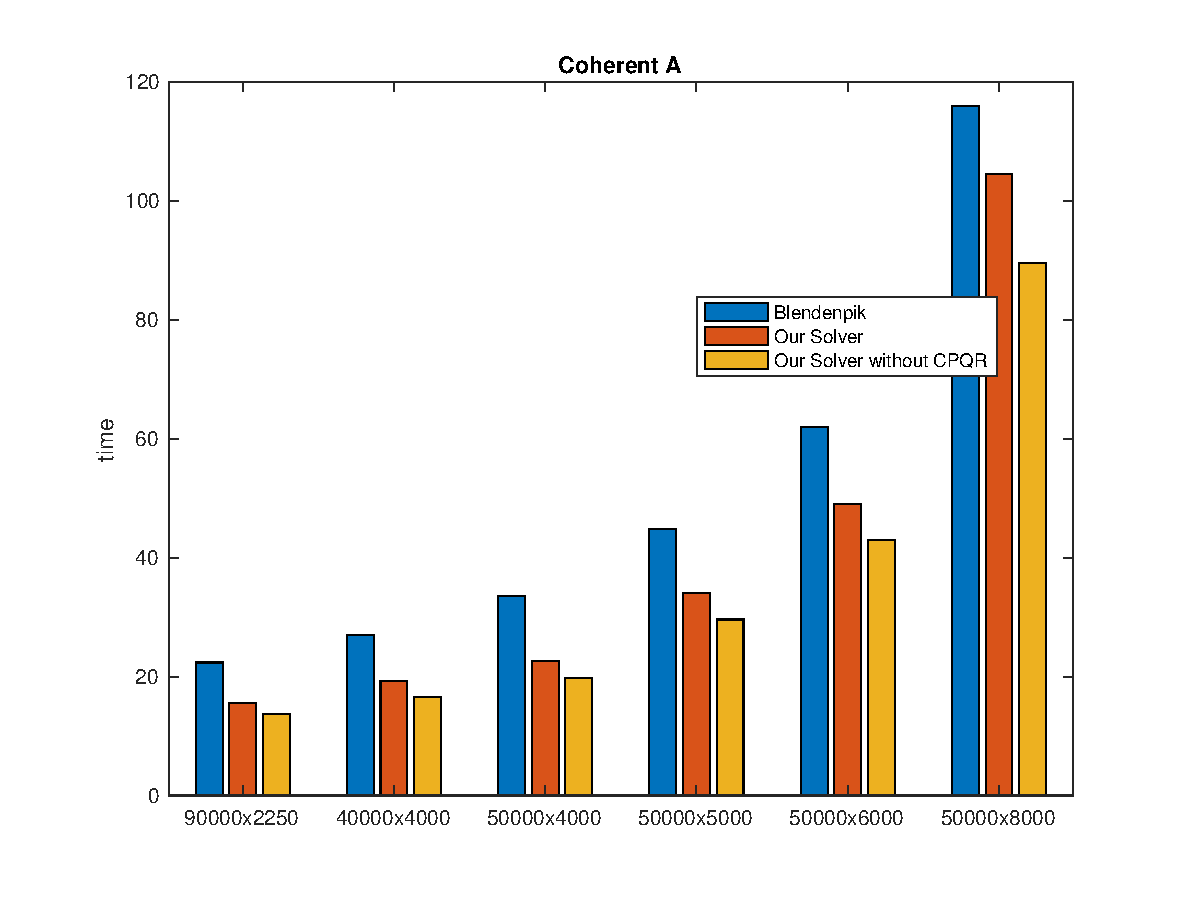
\includegraphics[width=\textwidth]{images/dense_co.eps} % first figure itself
        \caption{Time taken by solvers to compute the solution of problem (\ref{eq::problem}) for $A$ being (full rank) coherent dense matrices of various sizes (x-axis)}
        \label{fig::compare_blen_coherent}
    \end{minipage}\hfill
    \begin{minipage}{\mysize\textwidth}
        \centering
        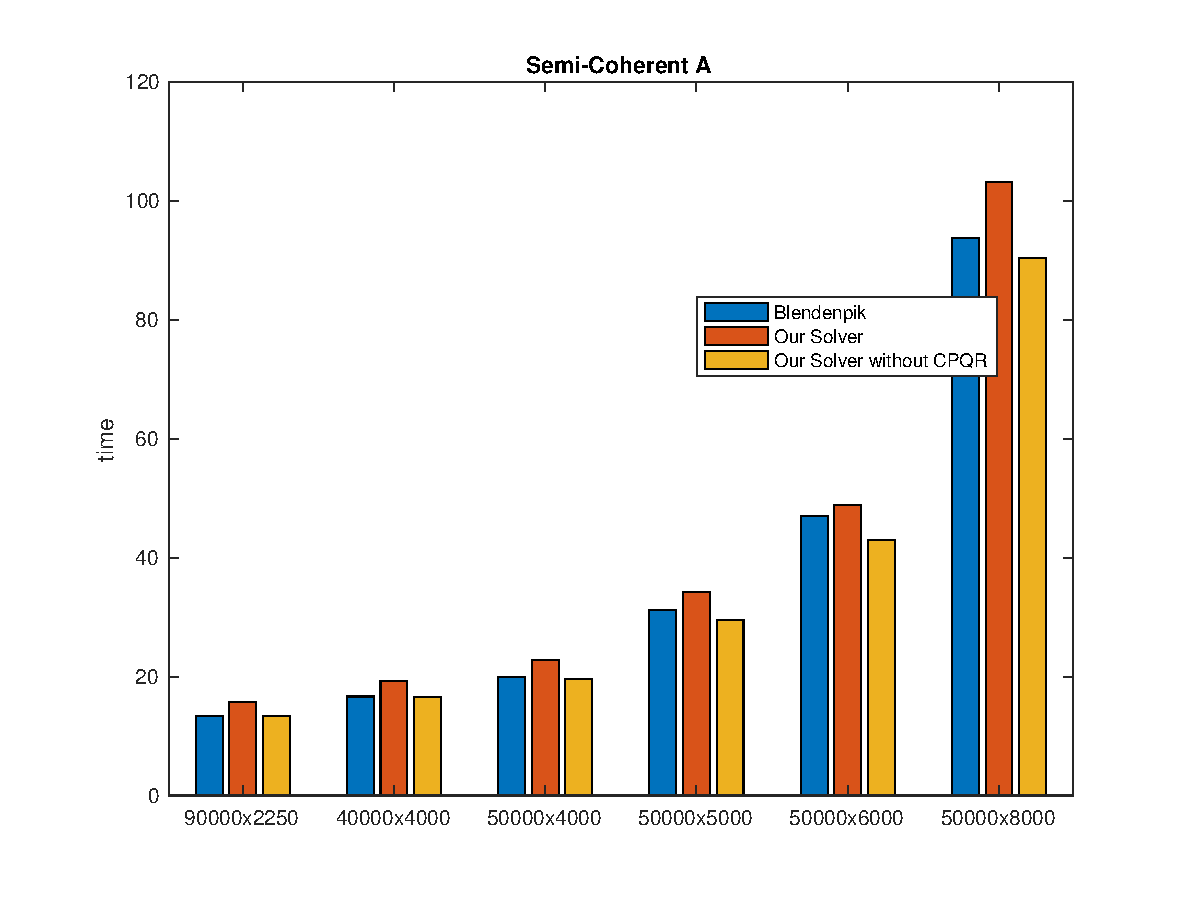
\includegraphics[width=\textwidth]{images/dense_semico.eps} % second figure itself
        \caption{Time taken by solvers to compute the solution of problem (\ref{eq::problem}) for $A$ being (full rank) semi-coherent dense matrices of various sizes (x-axis)}
        \label{fig::compare_blen_semi-coherent}
    \end{minipage}
    \begin{minipage}{\mysize\textwidth}
        \centering
        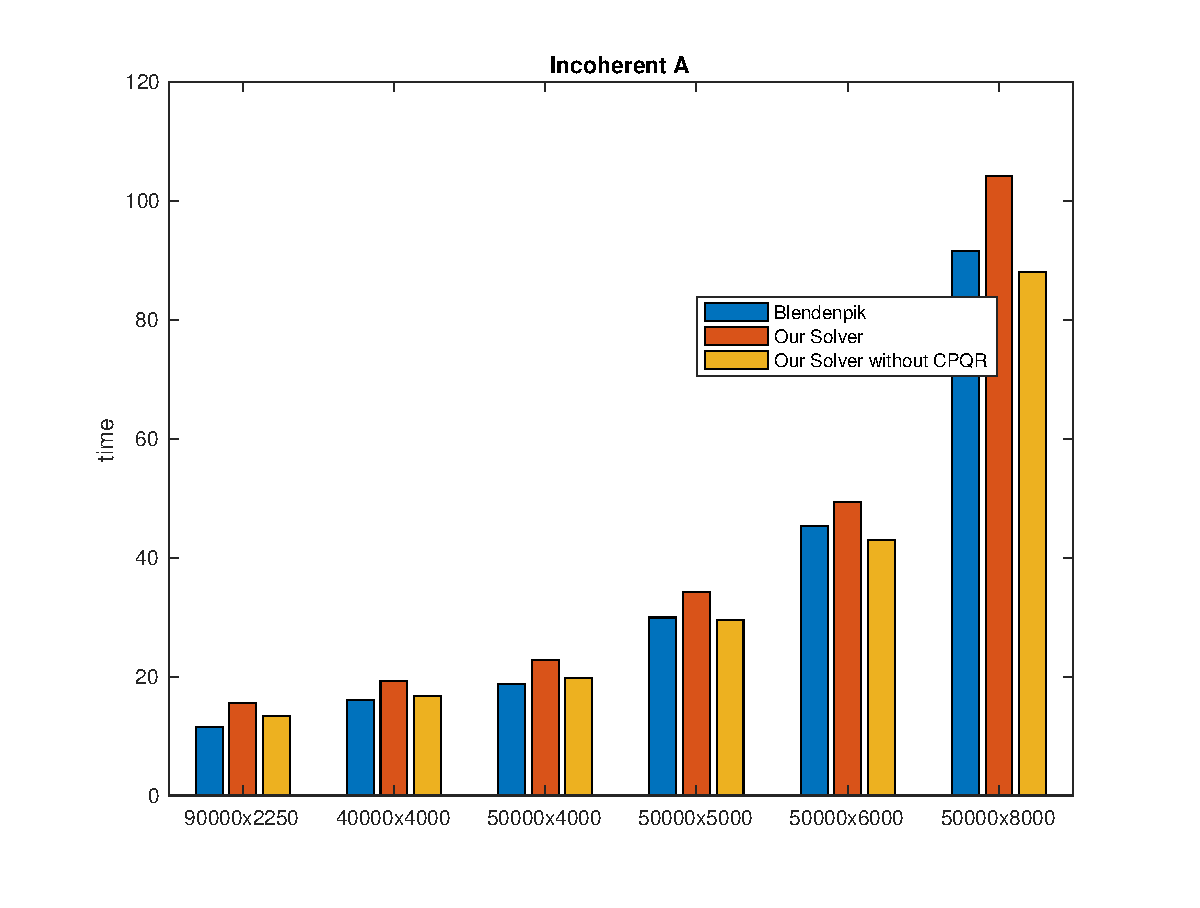
\includegraphics[width=\textwidth]{images/dense_inco.eps} % second figure itself
        \caption{Time taken by solvers to compute the solution of problem (\ref{eq::problem}) for $A$ being (full rank) incoherent dense matrices of various sizes (x-axis)}
        \label{fig::compare_blen_incoherent}
    \end{minipage}    
\end{figure}

\begin{figure}
\centering
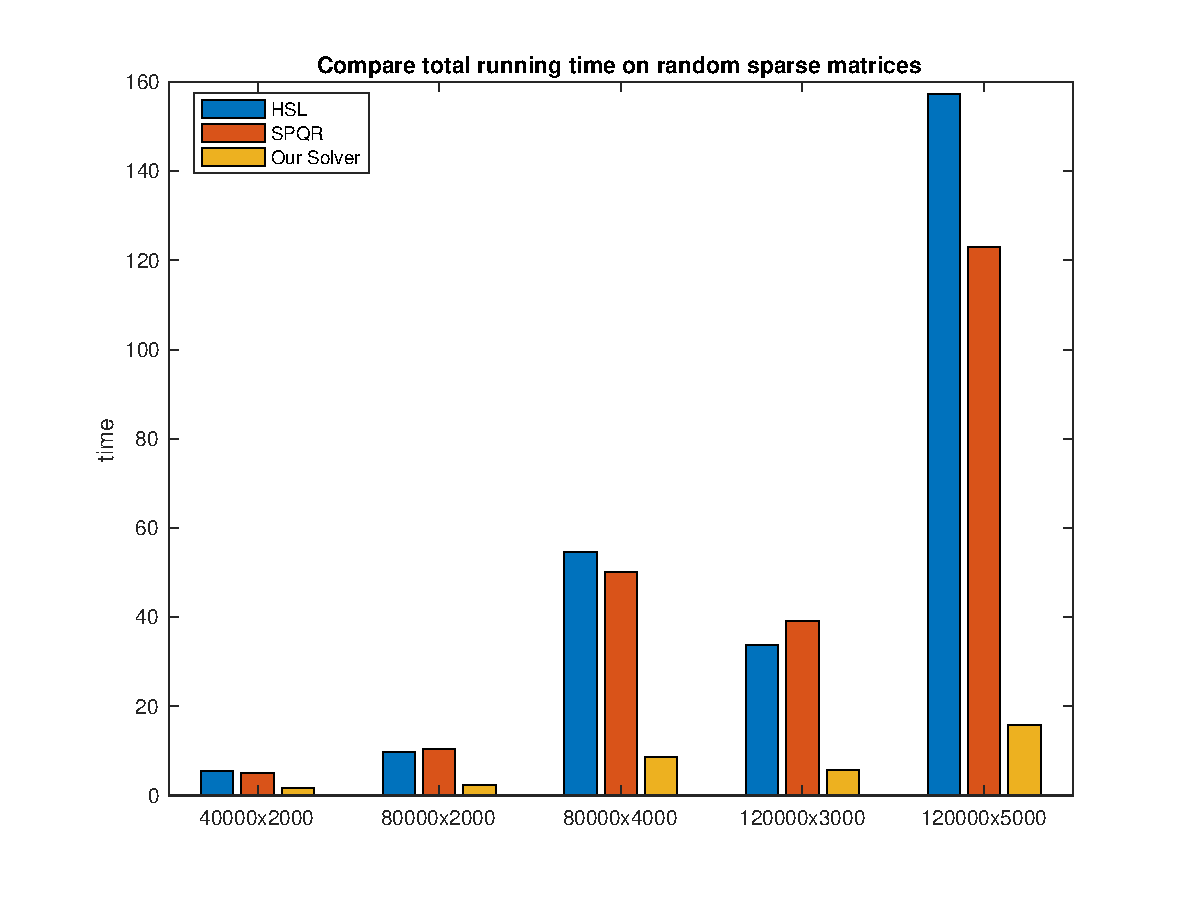
\includegraphics[width=0.6\textwidth]{images/random_sparse_inco.eps}
\caption{Our solver is much faster than state-of-the-arts LS_HSL and LS_SPQR on a range of random sparse data matrices.}
\label{fig::sparse_rand}
\end{figure}

\renewcommand{\mysize}{0.42}
\begin{figure}[]
    \centering
    \begin{minipage}{\mysize\textwidth}
        \centering
        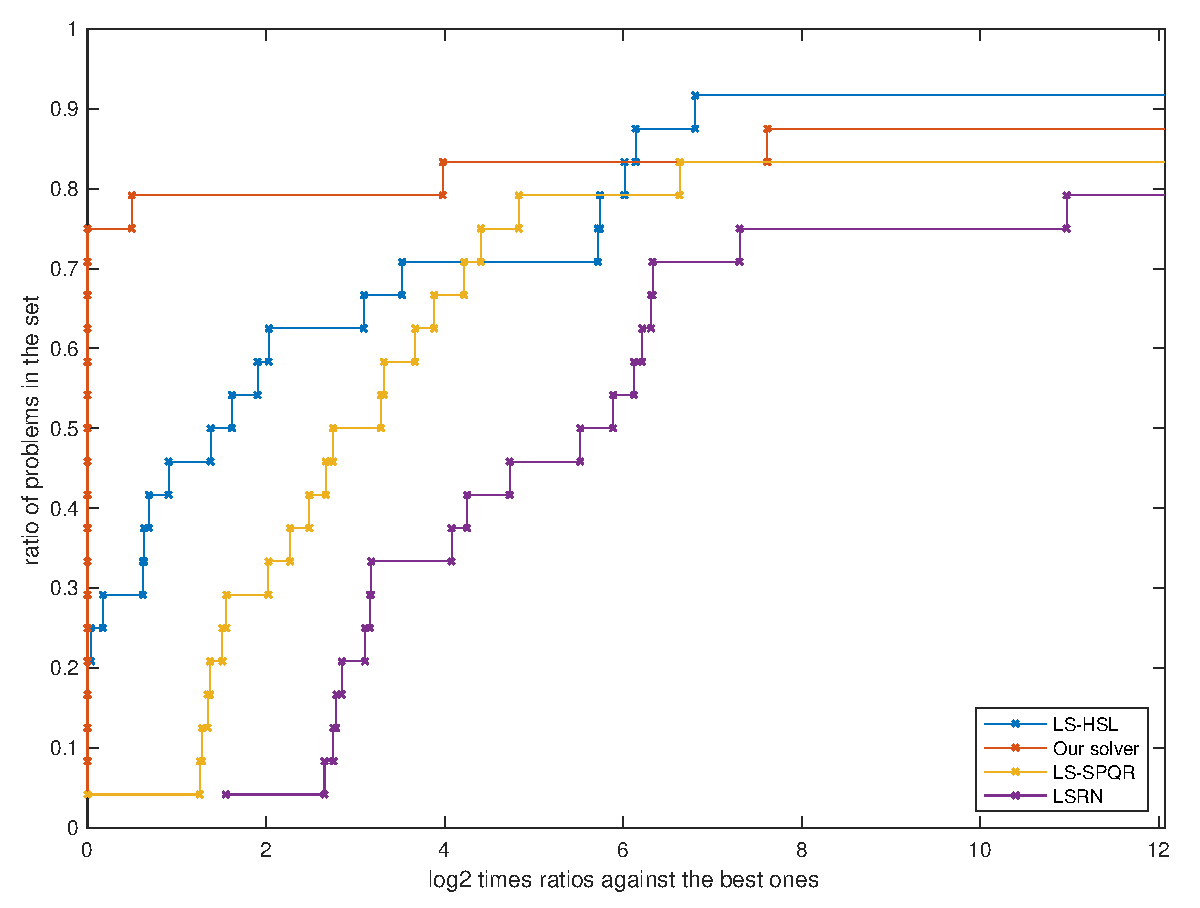
\includegraphics[width=\textwidth]{images/sparse_florida_all_30.eps} % first figure itself
        \caption{Performance profile comparison of Ski-LLS with LSRN, LS_HSL and LS_SPQR for all matrices $A\in\R^{n\times d}$ in the Florida matrix collection with $n\geq 30d$. }
        \label{fig::all_solver_30}
    \end{minipage}\hfill  
    \centering
    \begin{minipage}{\mysize\textwidth}
        \centering
        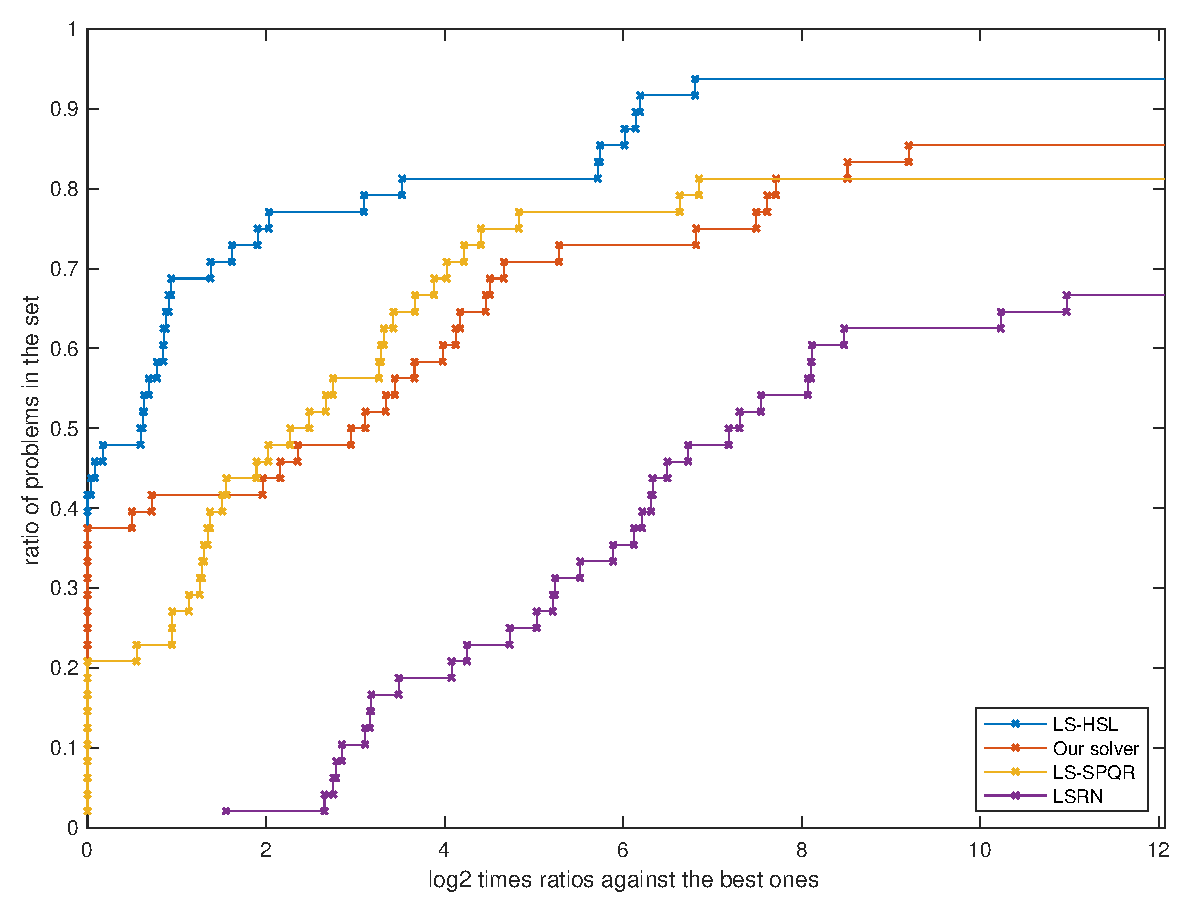
\includegraphics[width=\textwidth]{images/sparse_florida_all_10.eps} % first figure itself
        \caption{Performance profile comparison of Ski-LLS with LSRN, LS_HSL and LS_SPQR for all matrices $A\in\R^{n\times d}$ in the Florida matrix collection with $n\geq 10d$.}
        \label{fig::all_solver_10}
    \end{minipage}\hfill  
\end{figure}

\begin{figure}[]
    \centering
    \begin{minipage}{\mysize\textwidth}
        \centering
        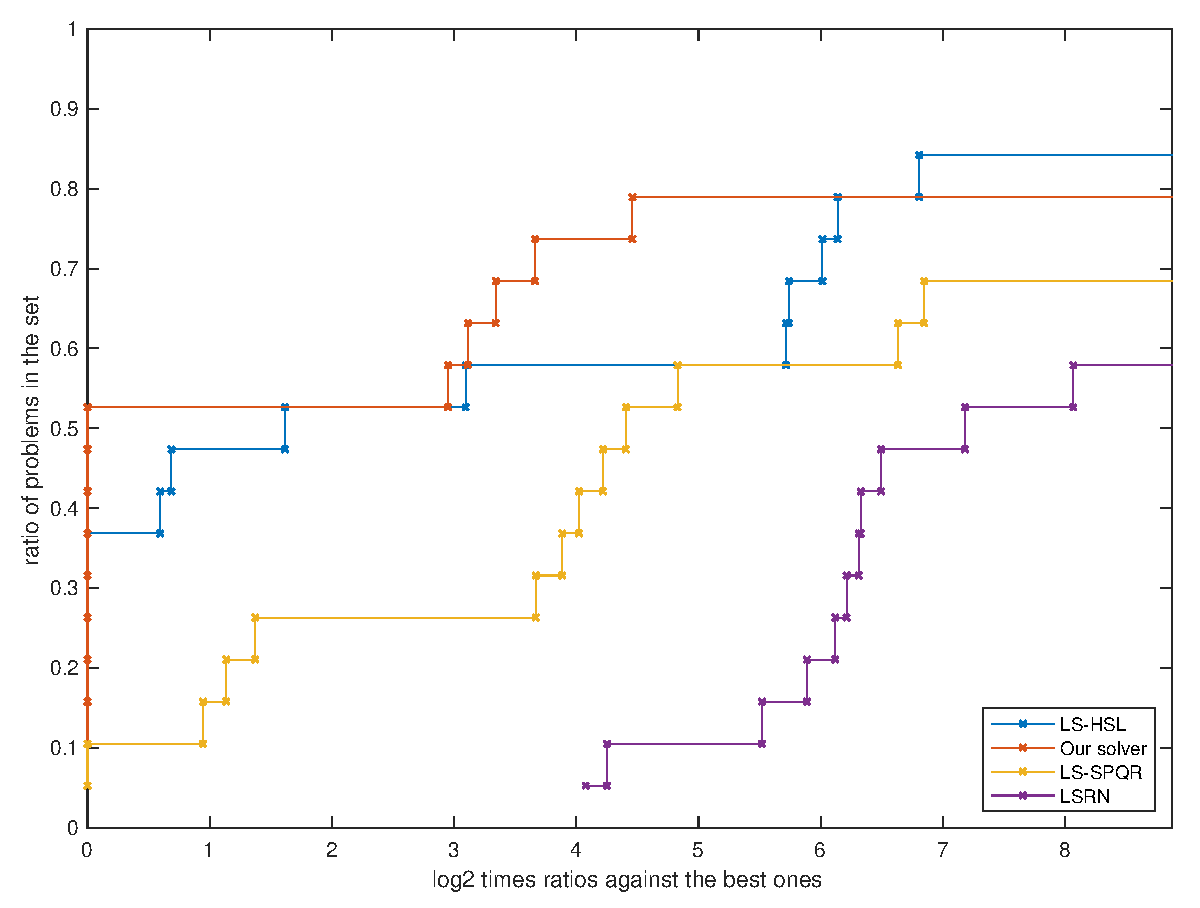
\includegraphics[width=\textwidth]{images/sparse_florida_lsqr_5_asp_10.eps} % first figure itself
        \caption{Performance profile comparison of Ski-LLS with LSRN, LS_HSL and LS_SPQR for all matrices $A\in\R^{n\times d}$ in the Florida matrix collection with $n\geq 10d$ and the unpreconditioned LSQR takes more than 5 seconds to solve.}
        \label{fig::all_solver_10_LSQR_5}
    \end{minipage}\hfill  
    \begin{minipage}{\mysize\textwidth}
    \centering
    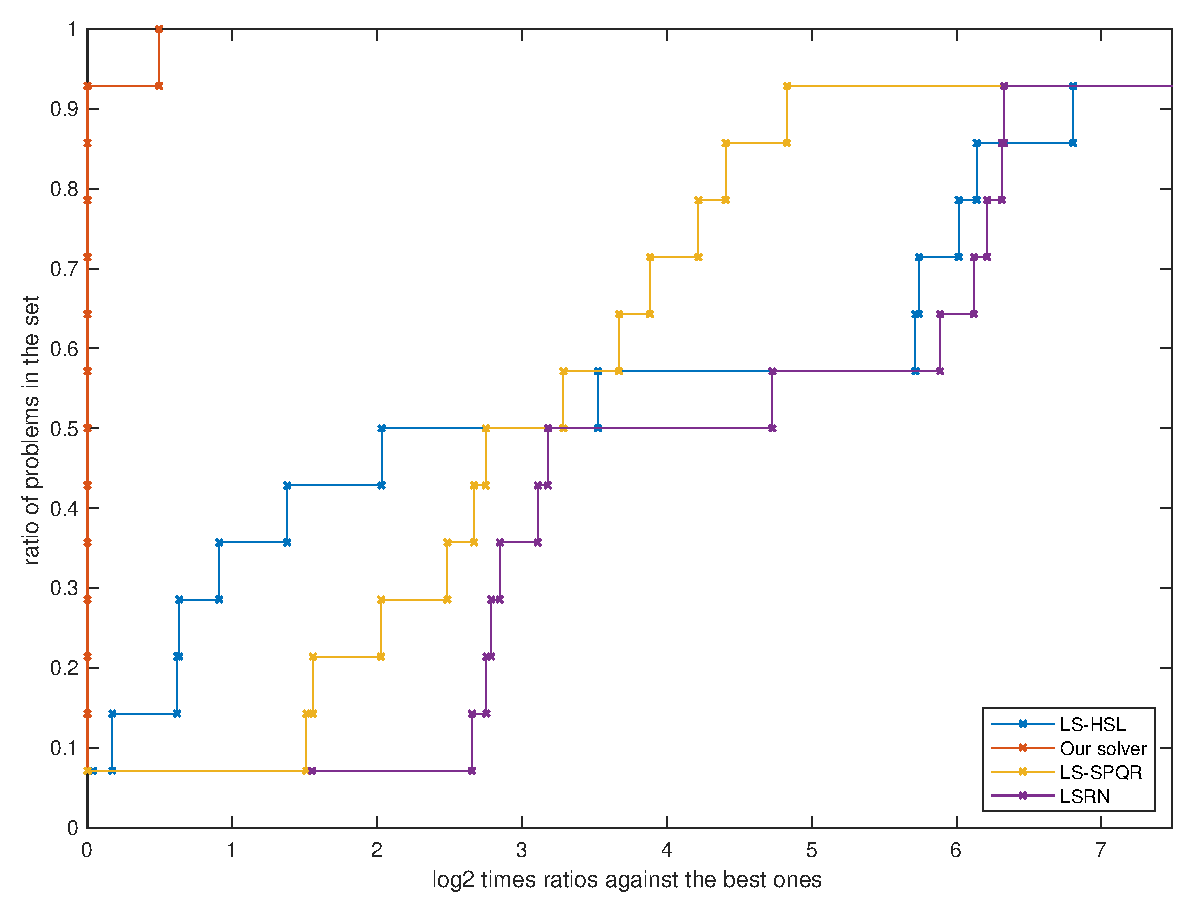
\includegraphics[width=\textwidth]{images/asp10_density_001.eps}
    \caption{All solvers, aspect ratio at least 10 and more than 1 percent number of non-zeros}
    \label{fig::density001}
    \end{minipage}

\end{figure}




\end{document}